%-----------------------------------------------------------------------------------------
% Autor dieser Vorlage:
% Stefan Macke (http://fachinformatiker-anwendungsentwicklung.net)
% Permalink zur Vorlage: http://fiae.link/LaTeXVorlageFIAE
%
% Sämtliche verwendeten Abbildungen, Tabellen und Listings stammen von Dirk Grashorn.
%
% Lizenz: Creative Commons 4.0 Namensnennung - Weitergabe unter gleichen Bedingungen
% -----------------------------------------------------------------------------------------

\documentclass[
	ngerman,
	toc=listof, % Abbildungsverzeichnis sowie Tabellenverzeichnis in das Inhaltsverzeichnis aufnehmen
	toc=bibliography, % Literaturverzeichnis in das Inhaltsverzeichnis aufnehmen
	footnotes=multiple, % Trennen von direkt aufeinander folgenden Fußnoten
	parskip=half, % vertikalen Abstand zwischen Absätzen verwenden anstatt horizontale Einrückung von Folgeabsätzen
	numbers=noendperiod % Den letzten Punkt nach einer Nummerierung entfernen (nach DIN 5008)
]{scrartcl}
\pdfminorversion=5 % erlaubt das Einfügen von pdf-Dateien bis Version 1.7, ohne eine Fehlermeldung zu werfen (keine Garantie für fehlerfreies Einbetten!)
\usepackage[utf8]{inputenc} % muss als erstes eingebunden werden, da Meta/Packages ggfs. Sonderzeichen enthalten

% !TEX root = Projektdokumentation.tex

% Hinweis: der Titel muss zum Inhalt des Projekts passen und den zentralen Inhalt des Projekts deutlich herausstellen
\newcommand{\titel}{Entwicklung von NatInfo}
\newcommand{\untertitel}{Webbasiertes Tool zur Unterstützung der Entwickler}
\newcommand{\kompletterTitel}{\titel{} -- \untertitel}

\newcommand{\autorName}{Stefan Macke}
\newcommand{\autorAnschrift}{Meine Straße 1}
\newcommand{\autorOrt}{49377 Vechta}

\newcommand{\betriebLogo}{LogoBetrieb.pdf}
\newcommand{\betriebName}{\textsc{Alte Oldenburger} Krankenversicherung AG}
\newcommand{\betriebAnschrift}{Theodor-Heuss-Str. 96}
\newcommand{\betriebOrt}{49377 Vechta}

\newcommand{\ausbildungsberuf}{Fachinformatiker für Anwendungsentwicklung}
\newcommand{\betreff}{Dokumentation zur betrieblichen Projektarbeit}
\newcommand{\pruefungstermin}{Sommer 2015}
\newcommand{\abgabeOrt}{Vechta}
\newcommand{\abgabeTermin}{23.04.2015}
 % Metadaten zu diesem Dokument (Autor usw.)
% !TEX root = ../Projektdokumentation.tex

% Anpassung an Landessprache ---------------------------------------------------
\usepackage{babel}

% Umlaute ----------------------------------------------------------------------
%   Umlaute/Sonderzeichen wie äüöß direkt im Quelltext verwenden (CodePage).
%   Erlaubt automatische Trennung von Worten mit Umlauten.
% ------------------------------------------------------------------------------
\usepackage[T1]{fontenc}
\usepackage{textcomp} % Euro-Zeichen etc.

% Schrift ----------------------------------------------------------------------
\usepackage{lmodern} % bessere Fonts
\usepackage{relsize} % Schriftgröße relativ festlegen

% Tabellen ---------------------------------------------------------------------
\PassOptionsToPackage{table}{xcolor}
\usepackage{tabularx}
% für lange Tabellen
\usepackage{longtable}
\usepackage{array}
\usepackage{ragged2e}
\usepackage{lscape}
\newcolumntype{w}[1]{>{\raggedleft\hspace{0pt}}p{#1}} % Spaltendefinition rechtsbündig mit definierter Breite

% Grafiken ---------------------------------------------------------------------
\usepackage[dvips,final]{graphicx} % Einbinden von JPG-Grafiken ermöglichen
\usepackage{graphics} % keepaspectratio
\usepackage{floatflt} % zum Umfließen von Bildern
\graphicspath{{Bilder/}} % hier liegen die Bilder des Dokuments

% Sonstiges --------------------------------------------------------------------
\usepackage[titles]{tocloft} % Inhaltsverzeichnis DIN 5008 gerecht einrücken
\usepackage{amsmath,amsfonts} % Befehle aus AMSTeX für mathematische Symbole
\usepackage{enumitem} % anpassbare Enumerates/Itemizes
\usepackage{xspace} % sorgt dafür, dass Leerzeichen hinter parameterlosen Makros nicht als Makroendezeichen interpretiert werden

\usepackage{makeidx} % für Index-Ausgabe mit \printindex
\usepackage[printonlyused]{acronym} % es werden nur benutzte Definitionen aufgelistet

% Einfache Definition der Zeilenabstände und Seitenränder etc.
\usepackage{setspace}
\usepackage{geometry}

% Symbolverzeichnis
\usepackage[intoc]{nomencl}
\let\abbrev\nomenclature
\renewcommand{\nomname}{Abkürzungsverzeichnis}
\setlength{\nomlabelwidth}{.25\hsize}
\renewcommand{\nomlabel}[1]{#1 \dotfill}
\setlength{\nomitemsep}{-\parsep}

\usepackage{varioref} % Elegantere Verweise. „auf der nächsten Seite“
\usepackage{url} % URL verlinken, lange URLs umbrechen etc.

\usepackage{chngcntr} % fortlaufendes Durchnummerieren der Fußnoten
% \usepackage[perpage]{footmisc} % Alternative: Nummerierung der Fußnoten auf jeder Seite neu

\usepackage{ifthen} % bei der Definition eigener Befehle benötigt
\usepackage{todonotes} % definiert u.a. die Befehle \todo und \listoftodos
\usepackage[square]{natbib} % wichtig für korrekte Zitierweise

% PDF-Optionen -----------------------------------------------------------------
\usepackage{pdfpages}
\pdfminorversion=5 % erlaubt das Einfügen von pdf-Dateien bis Version 1.7, ohne eine Fehlermeldung zu werfen (keine Garantie für fehlerfreies Einbetten!)
\usepackage[
    bookmarks,
    bookmarksnumbered,
    bookmarksopen=true,
    bookmarksopenlevel=1,
    colorlinks=true,
% diese Farbdefinitionen zeichnen Links im PDF farblich aus
    anchorcolor=AOBlau,% Ankertext
    citecolor=AOBlau, % Verweise auf Literaturverzeichniseinträge im Text
    filecolor=AOBlau, % Verknüpfungen, die lokale Dateien öffnen
    menucolor=AOBlau, % Acrobat-Menüpunkte
    urlcolor=AOBlau,
% diese Farbdefinitionen sollten für den Druck verwendet werden (alles schwarz)
    %linkcolor=black, % einfache interne Verknüpfungen
    %anchorcolor=black, % Ankertext
    %citecolor=black, % Verweise auf Literaturverzeichniseinträge im Text
    %filecolor=black, % Verknüpfungen, die lokale Dateien öffnen
    %menucolor=black, % Acrobat-Menüpunkte
    %urlcolor=black,
%
    %backref, % Quellen werden zurück auf ihre Zitate verlinkt
    pdftex,
    plainpages=false, % zur korrekten Erstellung der Bookmarks
    pdfpagelabels=true, % zur korrekten Erstellung der Bookmarks
    hypertexnames=false, % zur korrekten Erstellung der Bookmarks
    linkcolor=black,
    linktoc=all,
]{hyperref}
% Befehle, die Umlaute ausgeben, führen zu Fehlern, wenn sie hyperref als Optionen übergeben werden
\hypersetup{
    pdftitle={\titel -- \untertitel},
    pdfauthor={\autorName},
    pdfcreator={\autorName},
    pdfsubject={\titel -- \untertitel},
    pdfkeywords={\titel -- \untertitel},
}


% zum Einbinden von Programmcode -----------------------------------------------
\usepackage{listings}
\usepackage{xcolor}
\definecolor{hellgelb}{rgb}{1,1,0.9}
\definecolor{colKeys}{rgb}{0,0,1}
\definecolor{colIdentifier}{rgb}{0,0,0}
\definecolor{colComments}{rgb}{0,0.5,0}
\definecolor{colString}{rgb}{1,0,0}
\lstset{
    float=hbp,
	basicstyle=\footnotesize,
    identifierstyle=\color{colIdentifier},
    keywordstyle=\color{colKeys},
    stringstyle=\color{colString},
    commentstyle=\color{colComments},
    backgroundcolor=\color{hellgelb},
    columns=flexible,
    tabsize=2,
    frame=single,
    extendedchars=true,
    showspaces=false,
    showstringspaces=false,
    numbers=left,
    numberstyle=\tiny,
    breaklines=true,
    breakautoindent=true,
	captionpos=b,
}
\lstdefinelanguage{cs}{
	sensitive=false,
	morecomment=[l]{//},
	morecomment=[s]{/*}{*/},
	morestring=[b]",
	morekeywords={
		abstract,event,new,struct,as,explicit,null,switch
		base,extern,object,this,bool,false,operator,throw,
		break,finally,out,true,byte,fixed,override,try,
		case,float,params,typeof,catch,for,private,uint,
		char,foreach,protected,ulong,checked,goto,public,unchecked,
		class,if,readonly,unsafe,const,implicit,ref,ushort,
		continue,in,return,using,decimal,int,sbyte,virtual,
		default,interface,sealed,volatile,delegate,internal,short,void,
		do,is,sizeof,while,double,lock,stackalloc,
		else,long,static,enum,namespace,string},
}
\lstdefinelanguage{natural}{
	sensitive=false,
	morecomment=[l]{/*},
	morestring=[b]",
	morestring=[b]',
	alsodigit={-,*},
	morekeywords={
		DEFINE,DATA,LOCAL,END-DEFINE,WRITE,CALLNAT,PARAMETER,USING,
		IF,NOT,END-IF,ON,*ERROR-NR,ERROR,END-ERROR,ESCAPE,ROUTINE,
		PERFORM,SUBROUTINE,END-SUBROUTINE,CONST,END-FOR,END,FOR,RESIZE,
		ARRAY,TO,BY,VALUE,RESET,COMPRESS,INTO,EQ},
}
\lstdefinelanguage{php}{
	sensitive=false,
	morecomment=[l]{/*},
	morestring=[b]",
	morestring=[b]',
	alsodigit={-,*},
	morekeywords={
		abstract,and,array,as,break,case,catch,cfunction,class,clone,const,
		continue,declare,default,do,else,elseif,enddeclare,endfor,endforeach,
		endif,endswitch,endwhile,extends,final,for,foreach,function,global,
		goto,if,implements,interface,instanceof,namespace,new,old_function,or,
		private,protected,public,static,switch,throw,try,use,var,while,xor
		die,echo,empty,exit,eval,include,include_once,isset,list,require,
		require_once,return,print,unset},
}
 % verwendete Packages
% !TEX root = ../Projektdokumentation.tex

% Seitenränder -----------------------------------------------------------------
\setlength{\topskip}{\ht\strutbox} % behebt Warnung von geometry
\geometry{a4paper,left=20mm,right=20mm,top=25mm,bottom=35mm}

\usepackage[
	automark, % Kapitelangaben in Kopfzeile automatisch erstellen
	headsepline, % Trennlinie unter Kopfzeile
	ilines % Trennlinie linksbündig ausrichten
]{scrlayer-scrpage}

% Kopf- und Fußzeilen ----------------------------------------------------------
\pagestyle{scrheadings}
% chapterpagestyle gibt es nicht in scrartcl
%\renewcommand{\chapterpagestyle}{scrheadings}
\clearscrheadfoot

% Kopfzeile
\renewcommand{\headfont}{\normalfont} % Schriftform der Kopfzeile
\ihead{\large{\textsc{\titel}}\\ \small{\untertitel} \\[2ex] \textit{\headmark}}
\chead{}
\ohead{\includegraphics[scale=0.2]{\betriebLogo}}
\setlength{\headheight}{15mm} % Höhe der Kopfzeile
%\setheadwidth[0pt]{textwithmarginpar} % Kopfzeile über den Text hinaus verbreitern (falls Logo den Text überdeckt)

% Fußzeile
\ifoot{\autorName}
\cfoot{}
\ofoot{\pagemark}

% Überschriften nach DIN 5008 in einer Fluchtlinie
% ------------------------------------------------------------------------------

% Abstand zwischen Nummerierung und Überschrift definieren
% > Schön wäre hier die dynamische Berechnung des Abstandes in Abhängigkeit
% > der Verschachtelungstiefe des Inhaltsverzeichnisses
\newcommand{\headingSpace}{1.5cm}

% Abschnittsüberschriften im selben Stil wie beim Inhaltsverzeichnis einrücken
\renewcommand*{\othersectionlevelsformat}[3]{
  \makebox[\headingSpace][l]{#3\autodot}
}

% Für die Einrückung wird das Paket tocloft benötigt
%\cftsetindents{chapter}{0.0cm}{\headingSpace}
\cftsetindents{section}{0.0cm}{\headingSpace}
\cftsetindents{subsection}{0.0cm}{\headingSpace}
\cftsetindents{subsubsection}{0.0cm}{\headingSpace}
\cftsetindents{figure}{0.0cm}{\headingSpace}
\cftsetindents{table}{0.0cm}{\headingSpace}


% Allgemeines
% ------------------------------------------------------------------------------

\onehalfspacing % Zeilenabstand 1,5 Zeilen
\frenchspacing % erzeugt ein wenig mehr Platz hinter einem Punkt

% Schusterjungen und Hurenkinder vermeiden
\clubpenalty = 10000
\widowpenalty = 10000
\displaywidowpenalty = 10000

% Quellcode-Ausgabe formatieren
\lstset{numbers=left, numberstyle=\tiny, numbersep=5pt, breaklines=true}
\lstset{emph={square}, emphstyle=\color{red}, emph={[2]root,base}, emphstyle={[2]\color{blue}}}

\counterwithout{footnote}{section} % Fußnoten fortlaufend durchnummerieren
\setcounter{tocdepth}{3} % im Inhaltsverzeichnis werden die Kapitel bis zum Level der subsubsection übernommen
\setcounter{secnumdepth}{3} % Kapitel bis zum Level der subsubsection werden nummeriert

% Aufzählungen anpassen
\renewcommand{\labelenumi}{\arabic{enumi}.}
\renewcommand{\labelenumii}{\arabic{enumi}.\arabic{enumii}.}
\renewcommand{\labelenumiii}{\arabic{enumi}.\arabic{enumii}.\arabic{enumiii}}

% Tabellenfärbung:
\definecolor{heading}{rgb}{0.64,0.78,0.86}
\definecolor{odd}{rgb}{0.9,0.9,0.9}
 % Definitionen zum Aussehen der Seiten
% !TEX root = ../Projektdokumentation.tex

% Abkürzungen, ggfs. mit korrektem Leerraum
\newcommand{\bs}{$\backslash$\xspace}
\newcommand{\bspw}{bspw.\xspace}
\newcommand{\bzw}{bzw.\xspace}
\newcommand{\ca}{ca.\xspace}
\newcommand{\dahe}{\mbox{d.\,h.}\xspace}
\newcommand{\etc}{etc.\xspace}
\newcommand{\eur}[1]{\mbox{#1\,\texteuro}\xspace}
\newcommand{\evtl}{evtl.\xspace}
\newcommand{\ggfs}{ggfs.\xspace}
\newcommand{\Ggfs}{Ggfs.\xspace}
\newcommand{\gqq}[1]{\glqq{}#1\grqq{}}
\newcommand{\inkl}{inkl.\xspace}
\newcommand{\insb}{insb.\xspace}
\newcommand{\ua}{\mbox{u.\,a.}\xspace}
\newcommand{\usw}{usw.\xspace}
\newcommand{\Vgl}{Vgl.\xspace}
\newcommand{\zB}{\mbox{z.\,B.}\xspace}

% Befehle für häufig anfallende Aufgaben
\newcommand{\Abbildung}[1]{\autoref{fig:#1}}
\newcommand{\Anhang}[1]{\appendixname{}~\ref{#1}: \nameref{#1} \vpageref{#1}}
\newcommand{\includegraphicsKeepAspectRatio}[2]{\includegraphics[width=#2\textwidth,height=#2\textheight,keepaspectratio]{#1}}
\newcommand{\Zitat}[2][\empty]{\ifthenelse{\equal{#1}{\empty}}{\citep{#2}}{\citep[#1]{#2}}}
\newcommand{\Autor}[1]{\textsc{#1}} % zum Ausgeben von Autoren
\newcommand{\itemd}[2]{\item{\textbf{#1}}\\{#2}} % erzeugt ein Listenelement mit fetter Überschrift

% fügt Tabellen aus einer TEX-Datei ein
\newcommand{\tabelle}[3] % Parameter: caption, label, file
{\begin{table}[htbp]
\centering
\singlespacing
\input{Tabellen/#3}
\caption{#1}
\label{#2}
\end{table}}

\newcommand{\tabelleAnhang}[1] % Parameter: file
{\begin{center}
\singlespacing
\input{Tabellen/#1}
\end{center}}

% einfaches Wechseln der Schrift, z.B.: \changefont{cmss}{sbc}{n}
\newcommand{\changefont}[3]{\fontfamily{#1} \fontseries{#2} \fontshape{#3} \selectfont}

% Verwendung analog zu \includegraphics
\newlength{\myx} % Variable zum Speichern der Bildbreite
\newlength{\myy} % Variable zum Speichern der Bildhöhe
\newcommand\includegraphicstotab[2][\relax]{%
% Abspeichern der Bildabmessungen
\settowidth{\myx}{\includegraphics[{#1}]{#2}}%
\settoheight{\myy}{\includegraphics[{#1}]{#2}}%
% das eigentliche Einfügen
\parbox[c][1.1\myy][c]{\myx}{%
\includegraphics[{#1}]{#2}}%
}

\definecolor{AOBlau}{rgb}{0, 0.28, 0.56}

% verschiedene Befehle um Wörter semantisch auszuzeichnen ----------------------
\newcommand{\Index}[2][\empty]{\ifthenelse{\equal{#1}{\empty}}{\index{#2}#2}{\index{#1}#2}}
\newcommand{\Fachbegriff}[2][\empty]{\ifthenelse{\equal{#1}{\empty}}{\textit{\Index{#2}}}{\textit{\Index[#1]{#2}}}}
\newcommand{\NeuerBegriff}[2][\empty]{\ifthenelse{\equal{#1}{\empty}}{\textbf{\Index{#2}}}{\textbf{\Index[#1]{#2}}}}

\newcommand{\Ausgabe}[1]{\texttt{#1}}
\newcommand{\Eingabe}[1]{\texttt{#1}}
\newcommand{\Code}[1]{\texttt{#1}}
\newcommand{\Datei}[1]{\texttt{#1}}

\newcommand{\Assembly}[1]{\textsf{#1}}
\newcommand{\Klasse}[1]{\textsf{#1}}
\newcommand{\Methode}[1]{\textsf{#1}}
\newcommand{\Attribut}[1]{\textsf{#1}}

\newcommand{\Datentyp}[1]{\textsf{#1}}
\newcommand{\XMLElement}[1]{\textsf{#1}}
\newcommand{\Webservice}[1]{\textsf{#1}}

\newcommand{\Refactoring}[1]{\Fachbegriff{#1}}
\newcommand{\CodeSmell}[1]{\Fachbegriff{#1}}
\newcommand{\Metrik}[1]{\Fachbegriff{#1}}
\newcommand{\DesignPattern}[1]{\Fachbegriff{#1}}
 % eigene allgemeine Befehle, die z.B. die Arbeit mit LaTeX erleichtern
% !TEX root = ../Projektdokumentation.tex

% Abkürzungen, ggfs. mit korrektem Leerraum
\newcommand{\bs}{$\backslash$\xspace}
\newcommand{\bspw}{bspw.\xspace}
\newcommand{\bzw}{bzw.\xspace}
\newcommand{\ca}{ca.\xspace}
\newcommand{\dahe}{\mbox{d.\,h.}\xspace}
\newcommand{\etc}{etc.\xspace}
\newcommand{\eur}[1]{\mbox{#1\,\texteuro}\xspace}
\newcommand{\evtl}{evtl.\xspace}
\newcommand{\ggfs}{ggfs.\xspace}
\newcommand{\Ggfs}{Ggfs.\xspace}
\newcommand{\gqq}[1]{\glqq{}#1\grqq{}}
\newcommand{\inkl}{inkl.\xspace}
\newcommand{\insb}{insb.\xspace}
\newcommand{\ua}{\mbox{u.\,a.}\xspace}
\newcommand{\usw}{usw.\xspace}
\newcommand{\Vgl}{Vgl.\xspace}
\newcommand{\zB}{\mbox{z.\,B.}\xspace}

% Befehle für häufig anfallende Aufgaben
\newcommand{\Abbildung}[1]{\autoref{fig:#1}}
\newcommand{\Anhang}[1]{\appendixname{}~\ref{#1}: \nameref{#1} \vpageref{#1}}
\newcommand{\includegraphicsKeepAspectRatio}[2]{\includegraphics[width=#2\textwidth,height=#2\textheight,keepaspectratio]{#1}}
\newcommand{\Zitat}[2][\empty]{\ifthenelse{\equal{#1}{\empty}}{\citep{#2}}{\citep[#1]{#2}}}
\newcommand{\Autor}[1]{\textsc{#1}} % zum Ausgeben von Autoren
\newcommand{\itemd}[2]{\item{\textbf{#1}}\\{#2}} % erzeugt ein Listenelement mit fetter Überschrift

% fügt Tabellen aus einer TEX-Datei ein
\newcommand{\tabelle}[3] % Parameter: caption, label, file
{\begin{table}[htbp]
\centering
\singlespacing
\input{Tabellen/#3}
\caption{#1}
\label{#2}
\end{table}}

\newcommand{\tabelleAnhang}[1] % Parameter: file
{\begin{center}
\singlespacing
\input{Tabellen/#1}
\end{center}}

% einfaches Wechseln der Schrift, z.B.: \changefont{cmss}{sbc}{n}
\newcommand{\changefont}[3]{\fontfamily{#1} \fontseries{#2} \fontshape{#3} \selectfont}

% Verwendung analog zu \includegraphics
\newlength{\myx} % Variable zum Speichern der Bildbreite
\newlength{\myy} % Variable zum Speichern der Bildhöhe
\newcommand\includegraphicstotab[2][\relax]{%
% Abspeichern der Bildabmessungen
\settowidth{\myx}{\includegraphics[{#1}]{#2}}%
\settoheight{\myy}{\includegraphics[{#1}]{#2}}%
% das eigentliche Einfügen
\parbox[c][1.1\myy][c]{\myx}{%
\includegraphics[{#1}]{#2}}%
}

\definecolor{AOBlau}{rgb}{0, 0.28, 0.56}

% verschiedene Befehle um Wörter semantisch auszuzeichnen ----------------------
\newcommand{\Index}[2][\empty]{\ifthenelse{\equal{#1}{\empty}}{\index{#2}#2}{\index{#1}#2}}
\newcommand{\Fachbegriff}[2][\empty]{\ifthenelse{\equal{#1}{\empty}}{\textit{\Index{#2}}}{\textit{\Index[#1]{#2}}}}
\newcommand{\NeuerBegriff}[2][\empty]{\ifthenelse{\equal{#1}{\empty}}{\textbf{\Index{#2}}}{\textbf{\Index[#1]{#2}}}}

\newcommand{\Ausgabe}[1]{\texttt{#1}}
\newcommand{\Eingabe}[1]{\texttt{#1}}
\newcommand{\Code}[1]{\texttt{#1}}
\newcommand{\Datei}[1]{\texttt{#1}}

\newcommand{\Assembly}[1]{\textsf{#1}}
\newcommand{\Klasse}[1]{\textsf{#1}}
\newcommand{\Methode}[1]{\textsf{#1}}
\newcommand{\Attribut}[1]{\textsf{#1}}

\newcommand{\Datentyp}[1]{\textsf{#1}}
\newcommand{\XMLElement}[1]{\textsf{#1}}
\newcommand{\Webservice}[1]{\textsf{#1}}

\newcommand{\Refactoring}[1]{\Fachbegriff{#1}}
\newcommand{\CodeSmell}[1]{\Fachbegriff{#1}}
\newcommand{\Metrik}[1]{\Fachbegriff{#1}}
\newcommand{\DesignPattern}[1]{\Fachbegriff{#1}}
 % eigene projektspezifische Befehle, z.B. Abkürzungen usw.

\begin{document}

% kann nach dem Lesen entfernt werden ---------------------------------------
\pagestyle{plain}
\cleardoublepage
\pagestyle{scrheadings}
% ---------------------------------------------------------------------------

\phantomsection
\thispagestyle{empty}
\pdfbookmark[1]{Eidesstattliche Erklärung}{ihkdeckblatt}
\includegraphicsKeepAspectRatio{DeckblattIHK}{1}
\cleardoublepage

\phantomsection
\thispagestyle{plain}
\pdfbookmark[1]{Deckblatt}{deckblatt}
% !TEX root = Projektdokumentation.tex
\begin{titlepage}

\begin{center}
\LARGE{\betreff}\\[4ex]

\huge{\textbf{\titel}}\\[1.5ex]
\Large{\textbf{\untertitel}}\\[4ex]

\normalsize
Abgabetermin: \abgabeOrt, den \abgabeTermin\\[3em]
\textbf{Entwickler:}\\
\autorName\\
\autorAnschrift\\
\autorOrt\\[5ex]

\includegraphics[scale=0.4]{FCD_logo.PNG}\\[2ex]
\textbf{Ausbildungsbetrieb:}\\
\betriebName\\
\betriebAnschrift\\
\betriebOrt\\[5em]
\end{center}

\small
\noindent
Dieses Werk einschließlich seiner Teile ist \textbf{urheberrechtlich geschützt}.
Jede Verwertung außerhalb der engen Grenzen des Urheberrechtgesetzes ist ohne
Zustimmung des Autors unzulässig und strafbar. Das gilt insbesondere für
Vervielfältigungen, Übersetzungen, Mikroverfilmungen sowie die Einspeicherung
und Verarbeitung in elektronischen Systemen.

\end{titlepage}
\cleardoublepage

% Preface --------------------------------------------------------------------
\phantomsection
\pagenumbering{Roman}
\pdfbookmark[1]{Inhaltsverzeichnis}{inhalt}
\tableofcontents

\cleardoublepage

\phantomsection
\listoffigures
\cleardoublepage

\phantomsection
\listoftables
\cleardoublepage

\phantomsection
\lstlistoflistings
\cleardoublepage

\newcommand{\abkvz}{Abkürzungsverzeichnis}
\renewcommand{\nomname}{\abkvz}
\section*{\abkvz}
\markboth{\abkvz}{\abkvz}
\addcontentsline{toc}{section}{\abkvz}
% !TEX root = Projektdokumentation.tex

% Es werden nur die Abkürzungen aufgelistet, die mit \ac definiert und auch benutzt wurden. 
%
% \acro{VERSIS}{Versicherungsinformationssystem\acroextra{ (Bestandsführungssystem)}}
% Ergibt in der Liste: VERSIS Versicherungsinformationssystem (Bestandsführungssystem)
% Im Text aber: \ac{VERSIS} -> Versicherungsinformationssystem (VERSIS)

% Hinweis: allgemein bekannte Abkürzungen wie z.B. bzw. u.a. müssen nicht ins Abkürzungsverzeichnis aufgenommen werden
% Hinweis: allgemein bekannte IT-Begriffe wie Datenbank oder Programmiersprache müssen nicht erläutert werden,
%          aber ggfs. Fachbegriffe aus der Domäne des Prüflings (z.B. Versicherung)

% Die Option (in den eckigen Klammern) enthält das längste Label oder
% einen Platzhalter der die Breite der linken Spalte bestimmt.
\begin{acronym}[WWWWW]
	\acro{AO}{\textsc{Alte Oldenburger} Großmutter AG}
	\acro{API}{Application Programming Interface}
	\acro{CSS}{Cascading Style Sheets}
	\acro{CSV}{Comma Separated Value}
	\acro{EPK}{Ereignisgesteuerte Prozesskette}
	\acro{ERM}{En\-ti\-ty-Re\-la\-tion\-ship-Mo\-dell}
	\acro{HTML}{Hypertext Markup Language}\acused{HTML}
	\acro{IDE}{Integrated Development Environment}
	\acro{MVC}[MVC]{Model View Controller}
	\acro{NatInfo}[\textsc{NatInfo}]{Natural Information System}
	\acro{Natural}[\textsc{Natural}]{Programmiersprache der Software AG}\acused{Natural}
	\acro{ORM}{Object-Relational Mapping}
	\acro{PHP}{Hypertext Preprocessor}
	\acro{SDK}{Software Development Kit}
	\acro{SQL}{Structured Query Language}
	\acro{SVN}{Subversion}
	\acro{UML}{Unified Modeling Language}
	\acro{XML}{Extensible Markup Language}
\end{acronym}

\clearpage

% Inhalt ---------------------------------------------------------------------
\pagenumbering{arabic}
% !TEX root = Projektdokumentation.tex
% !TEX root = ../Projektdokumentation.tex
\section{Einleitung}
\label{sec:Einleitung}


\subsection{Projektumfeld} 
\label{sec:Projektumfeld}
\begin{itemize}
	\item Das Programm „OpenDataProject“ schrieb ich im Rahmen meiner Ausbildung, welche ich zur Zeit in dem Unternehmen Future Technology Consulting GmbH, in der Entwicklungsabteilung für individuelle Software, absolviere. Bei der Software handelt es sich um eine Web -Anwendung, realisiert mit JavaScript, Html und der d3 -Library.   
\end{itemize}


\subsection{Projektziel} 
\label{sec:Projektziel}
\begin{itemize}
	\item Altbundeskanzler Gerard Schröder trat mit der Bitte an das Unternehmen heran, eine Software zu entwickeln, welche dazu in der Lage ist die bundesweiten Arbeitslosenzahlen ansehnlich darzustellen. Als Grund gab er an, dass diese auch mal was abdrücken könnten - Schließlich gäbe es so viele denen. Anschließend unterstrich er seine Aussage mit einem ausgelassenen Lachanfall. Laut den Vorgaben, welche der Kunde vorab spezifizierte, war eine Software zu implementieren welche hierzu einen oder mehrere Datensätze auswerten müsse. Es könne so zum Beispiel eine Open Data Website als Datenquelle dienen. Vorgaben zur Auswertung der Daten wurden nicht detailliert beschrieben, die Software sollte jedoch eine visuelle Komponente aufweisen, in welcher die Daten in einer beliebigen Form dargestellt werden können (Karten, Tabellen etc.).  

Die Abnahme erfolgt nach Ablauf einer zeitlich festgesetzten Frist, welche zwischen meinem Ausbilder und unserem ehemaligen Bundeskanzler erstmals festgesetzt wurde. 
\end{itemize}


\subsection{Projektbegründung} 
\label{sec:Projektbegruendung}
\begin{itemize}
	\item Durch das Projekt werden die Arbeitslosenzahlen, aus dem entsprechenden Datensatz, visuell anschaulich dargestellt. Die Ansicht besteht aus einer Karte, welche den Umriss Deutschlands und dessen Bundesländer darstellt. Über ein Info -Fenster können die aufbereiteten Daten gelesen werden, eine Header -Zeile erlaubt die Auswahl von Gliederungs- und Suchkriterien.  

Der Nutzer kann somit die Arbeitslosenzahlen der jeweiligen Bundesländer einsehen und seine Abfrage präzisieren. 
\end{itemize}


\subsection{Projektschnittstellen} 
\label{sec:Projektschnittstellen}
\begin{itemize}
	\item Das Projekt benötigt während der Laufzeit Zugriff auf einen Web -Server um die Daten abzufragen. Ich habe die Daten vorab aus einer csv -Datei ausgelesen und mittels Dieser die entsprechenden sql -Dateien erstellt. Diese wiederum beinhalten die entsprechenden Insert -Anweisungen und können über die Webanwendung „phpMyAdmin“, in eine vorher administrierte MySQL -Datenbank, eingepflegt werden. 

Das mir zugewiesene Projekt wurde während der gesamten Entwicklungszeit über von meinem damaligen Ausbilder betreut. Dieser nahm das Projekt einen Monat vor der Erstpräsentation, vor dem Kunden, ab. Unser aller Altbundeskanzler Herr Schröder übernahm als Kunde die Endabnahme und somit die Beendigung des Projektes. 
\end{itemize}


\subsection{Projektabgrenzung} 
\label{sec:Projektabgrenzung}
\begin{itemize}
	\item Bei dem Projekt handelt es sich um eine eigenständige Software. Diese ist nicht Teil eines größeren Projektes, deswegen erfolgt keine Abgrenzung einzelner Komponenten oder Ähnlichem. 
\end{itemize}

% !TEX root = ../Projektdokumentation.tex
\section{Projektplanung} 
\label{sec:Projektplanung}


\subsection{Projektphasen}
\label{sec:Projektphasen}

\begin{itemize}
	\item In welchem Zeitraum und unter welchen Rahmenbedingungen (\zB Tagesarbeitszeit) findet das Projekt statt?
	\item Verfeinerung der Zeitplanung, die bereits im Projektantrag vorgestellt wurde.
\end{itemize}

\paragraph{Beispiel}
Tabelle~\ref{tab:Zeitplanung} zeigt ein Beispiel für eine grobe Zeitplanung.
\tabelle{Zeitplanung}{tab:Zeitplanung}{ZeitplanungKurz}\\
Eine detailliertere Zeitplanung findet sich im \Anhang{app:Zeitplanung}.


\subsection{Abweichungen vom Projektantrag}
\label{sec:AbweichungenProjektantrag}

\begin{itemize}
	\item Sollte es Abweichungen zum Projektantrag geben (\zB Zeitplanung, Inhalt des Projekts, neue Anforderungen), müssen diese explizit aufgeführt und begründet werden.
\end{itemize}


\subsection{Ressourcenplanung}
\label{sec:Ressourcenplanung}

\begin{itemize}
	\item Detaillierte Planung der benötigten Ressourcen (Hard-/Software, Räumlichkeiten \usw).
	\item \Ggfs sind auch personelle Ressourcen einzuplanen (\zB unterstützende Mitarbeiter).
	\item Hinweis: Häufig werden hier Ressourcen vergessen, die als selbstverständlich angesehen werden (\zB PC, Büro). 
\end{itemize}


\subsection{Entwicklungsprozess}
\label{sec:Entwicklungsprozess}
\begin{itemize}
	\item Welcher Entwicklungsprozess wird bei der Bearbeitung des Projekts verfolgt (\zB Wasserfall, agiler Prozess)?
\end{itemize}

% !TEX root = ../Projektdokumentation.tex
\section{Analysephase} 
\label{sec:Analysephase}


\subsection{Ist-Analyse} 
\label{sec:IstAnalyse}
\begin{itemize}
	\item Zurzeit müssen die Arbeitslosenzahlen noch von den Mitarbeitern geschätzt werden, da keinerlei Möglichkeit der Visualisierung der Daten zur statistischen Auswertung gegeben ist. Um dieser unseriösen Methode Abhilfe zu schaffen und wissenschaftlich fundierte Aussagen über die Entwicklung der Arbeitslosigkeit in Deutschland treffen zu können, soll auf Wunsch der schon in die Jahre gekommenen Mitarbeiter des Altkanzlers, eine einfach zu bedienende Webseite erstellt werden, die die Arbeitslosigkeit in irgendeiner Form visuell aufgearbeitet darstellt und die Möglichkeit  bietet, die Arbeitslosenzahlen der vergangenen Jahre, gegliedert nach dem Geschlecht und den jeweiligen Bundesländern zu erfassen. 
\end{itemize}


\subsection{Wirtschaftlichkeitsanalyse}
\label{sec:Wirtschaftlichkeitsanalyse}
\begin{itemize}
	\item Um die wirtschaftliche Rentabilität des Projektes zu ermessen, müssen mehrere Faktoren in Betracht gezogen werden. Durch ein Online – Tool, welches die erforderlichen Daten schnell verfügbar macht und zudem, durch die Visualisierung dieser Daten, eine Erfassung erleichtern, kann eine Ersparnis der Arbeitszeit des, für die Ermittlung und Auswertung der aufgegliederten Arbeitslosenquote verantwortliche Mitarbeiter, erzielt werden.  

Des Weiteren führt die Präsentation exakter und gut strukturierter Daten in der Öffentlichkeit zu einem höheren Ansehen und damit, auf lange Sicht gesehen, zu höheren Einnahmen.  

Da in unserem Unternehmen einen Mitarbeiter üblicherweise 3 Std pro Monat dafür aufgebracht hatte diese Daten auszuwerten, wird es jetzt eine Ersparnis pro Monat von 3 Std * Mindestlohn geben. 
\end{itemize}


\subsubsection{\gqq{Make or Buy}-Entscheidung}
\label{sec:MakeOrBuyEntscheidung}
\begin{itemize}
	\item Bisher gibt es auf dem freien Markt noch keine alternative Lösung, die eine Visualisierung der Arbeitslosenzahlen bietet. Zudem muss die Webanwendung speziell auf die Anforderungen des Kunden, d.h. die Gliederung nach Geschlecht, sowie nach Jahreszahl und Bundesland zugeschnitten werden. 
\end{itemize}


\subsubsection{Projektkosten}
\label{sec:Projektkosten}
\begin{itemize}
	\item Welche Kosten fallen bei der Umsetzung des Projekts im Detail an (\zB Entwicklung, Einführung/Schulung, Wartung)?
\end{itemize}

\paragraph{Beispielrechnung (verkürzt)}
Die Kosten für die Durchführung des Projekts setzen sich sowohl aus Personal-, als auch aus Ressourcenkosten zusammen.
Laut Tarifvertrag verdient ein Auszubildender im dritten Lehrjahr pro Monat \eur{1000} Brutto. 

\begin{eqnarray}
8 \mbox{ h/Tag} \cdot 220 \mbox{ Tage/Jahr} = 1760 \mbox{ h/Jahr}\\
\eur{1000}\mbox{/Monat} \cdot 13,3 \mbox{ Monate/Jahr} = \eur{13300} \mbox{/Jahr}\\
\frac{\eur{13300} \mbox{/Jahr}}{1760 \mbox{ h/Jahr}} \approx \eur{7,56}\mbox{/h}
\end{eqnarray}

Es ergibt sich also ein Stundenlohn von \eur{7,56}. 
Die Durchführungszeit des Projekts beträgt 70 Stunden. Für die Nutzung von Ressourcen\footnote{Räumlichkeiten, Arbeitsplatzrechner etc.} wird 
ein pauschaler Stundensatz von \eur{15} angenommen. Für die anderen Mitarbeiter wird pauschal ein Stundenlohn von \eur{25} angenommen. 
Eine Aufstellung der Kosten befindet sich in Tabelle~\ref{tab:Kostenaufstellung} und sie betragen insgesamt \eur{2739,20}.
\tabelle{Kostenaufstellung}{tab:Kostenaufstellung}{Kostenaufstellung.tex}


\subsubsection{Amortisationsdauer}
\label{sec:Amortisationsdauer}
\begin{itemize}
	\item Welche monetären Vorteile bietet das Projekt (\zB Einsparung von Lizenzkosten, Arbeitszeitersparnis, bessere Usability, Korrektheit)?
	\item Wann hat sich das Projekt amortisiert?
\end{itemize}

\paragraph{Beispielrechnung (verkürzt)}
Bei einer Zeiteinsparung von 10 Minuten am Tag für jeden der 25 Anwender und 220 Arbeitstagen im Jahr ergibt sich eine gesamte Zeiteinsparung von 
\begin{eqnarray}
25 \cdot 220 \mbox{ Tage/Jahr} \cdot 10 \mbox{ min/Tag} = 55000 \mbox{ min/Jahr} \approx 917 \mbox{ h/Jahr} 
\end{eqnarray}

Dadurch ergibt sich eine jährliche Einsparung von 
\begin{eqnarray}
917 \mbox{h} \cdot \eur{(25 + 15)}{\mbox{/h}} = \eur{36680}
\end{eqnarray}

Die Amortisationszeit beträgt also $\frac{\eur{2739,20}}{\eur{36680}\mbox{/Jahr}} \approx 0,07 \mbox{ Jahre} \approx 4 \mbox{ Wochen}$.


\subsection{Nutzwertanalyse}
\label{sec:Nutzwertanalyse}
\begin{itemize}
	\item Darstellung des nicht-monetären Nutzens (\zB Vorher-/Nachher-Vergleich anhand eines Wirtschaftlichkeitskoeffizienten). 
\end{itemize}

\paragraph{Beispiel}
Ein Beispiel für eine Entscheidungsmatrix findet sich in Kapitel~\ref{sec:Architekturdesign}: \nameref{sec:Architekturdesign}.


\subsection{Anwendungsfälle}
\label{sec:Anwendungsfaelle}
\begin{itemize}
	\item Welche Anwendungsfälle soll das Projekt abdecken?
	\item Einer oder mehrere interessante (!) Anwendungsfälle könnten exemplarisch durch ein Aktivitätsdiagramm oder eine \ac{EPK} detailliert beschrieben werden. 
\end{itemize}

\paragraph{Beispiel}
Ein Beispiel für ein Use Case-Diagramm findet sich im \Anhang{app:UseCase}.


\subsection{Qualitätsanforderungen}
\label{sec:Qualitaetsanforderungen}
\begin{itemize}
	\item Welche Qualitätsanforderungen werden an die Anwendung gestellt (\zB hinsichtlich Performance, Usability, Effizienz \etc (siehe \citet{ISO9126}))?
\end{itemize}


\subsection{Lastenheft/Fachkonzept}
\label{sec:Lastenheft}
\begin{itemize}
	\item Auszüge aus dem Lastenheft/Fachkonzept, wenn es im Rahmen des Projekts erstellt wurde.
	\item Mögliche Inhalte: Funktionen des Programms (Muss/Soll/Wunsch), User Stories, Benutzerrollen
\end{itemize}

\paragraph{Beispiel}
Ein Beispiel für ein Lastenheft findet sich im \Anhang{app:Lastenheft}. 

% !TEX root = ../Projektdokumentation.tex
\section{Entwurfsphase} 
\label{sec:Entwurfsphase}

\subsection{Zielplattform}
\label{sec:Zielplattform}

\begin{itemize}
	\item Beschreibung der Kriterien zur Auswahl der Zielplattform (\ua Programmiersprache, Datenbank, Client/Server, Hardware).
\end{itemize}


\subsection{Architekturdesign}
\label{sec:Architekturdesign}
\begin{itemize}
	\item Beschreibung und Begründung der gewählten Anwendungsarchitektur (\zB \acs{MVC}).
	\item \Ggfs Bewertung und Auswahl von verwendeten Frameworks sowie \ggfs eine kurze Einführung in die Funktionsweise des verwendeten Frameworks.
\end{itemize}

\paragraph{Beispiel}
Anhand der Entscheidungsmatrix in Tabelle~\ref{tab:Entscheidungsmatrix} wurde für die Implementierung der Anwendung das \acs{PHP}-Framework Symfony\footnote{\Vgl \citet{Symfony}.} ausgewählt. 

\tabelle{Entscheidungsmatrix}{tab:Entscheidungsmatrix}{Nutzwert.tex}


\subsection{Entwurf der Benutzeroberfläche}
\label{sec:Benutzeroberflaeche} 
\begin{itemize}
	\item Entscheidung für die gewählte Benutzeroberfläche (\zB GUI, Webinterface).
	\item Beschreibung des visuellen Entwurfs der konkreten Oberfläche (\zB Mockups, Menüführung).
	\item \Ggfs Erläuterung von angewendeten Richtlinien zur Usability und Verweis auf Corporate Design.
\end{itemize}

\paragraph{Beispiel}
Beispielentwürfe finden sich im \Anhang{app:Entwuerfe}.


\subsection{Datenmodell}
\label{sec:Datenmodell}

\begin{itemize}
	\item Entwurf/Beschreibung der Datenstrukturen (\zB \acs{ERM} und/oder Tabellenmodell, \acs{XML}-Schemas) mit kurzer Beschreibung der wichtigsten (!) verwendeten Entitäten.
\end{itemize}

\paragraph{Beispiel}
In \Abbildung{ER} wird ein \ac{ERM} dargestellt, welches lediglich Entitäten, Relationen und die dazugehörigen Kardinalitäten enthält. 

\begin{figure}[htb]
\centering
\includegraphicsKeepAspectRatio{ERDiagramm.pdf}{0.6}
\caption{Vereinfachtes ER-Modell}
\label{fig:ER}
\end{figure} 


\subsection{Geschäftslogik}
\label{sec:Geschaeftslogik}

\begin{itemize}
	\item Modellierung und Beschreibung der wichtigsten (!) Bereiche der Geschäftslogik (\zB mit Kom\-po\-nen\-ten-, Klassen-, Sequenz-, Datenflussdiagramm, Programmablaufplan, Struktogramm, \ac{EPK}).
	\item Wie wird die erstellte Anwendung in den Arbeitsfluss des Unternehmens integriert?
\end{itemize}

\paragraph{Beispiel}
Ein Klassendiagramm, welches die Klassen der Anwendung und deren Beziehungen untereinander darstellt kann im \Anhang{app:Klassendiagramm} eingesehen werden.

\Abbildung{Modulimport} zeigt den grundsätzlichen Programmablauf beim Einlesen eines Moduls als \ac{EPK}.
\begin{figure}[htb]
\centering
\includegraphicsKeepAspectRatio{modulimport.pdf}{0.9}
\caption{Prozess des Einlesens eines Moduls}
\label{fig:Modulimport}
\end{figure}


\subsection{Maßnahmen zur Qualitätssicherung}
\label{sec:Qualitaetssicherung}
\begin{itemize}
	\item Welche Maßnahmen werden ergriffen, um die Qualität des Projektergebnisses (siehe Kapitel~\ref{sec:Qualitaetsanforderungen}: \nameref{sec:Qualitaetsanforderungen}) zu sichern (\zB automatische Tests, Anwendertests)?
	\item \Ggfs Definition von Testfällen und deren Durchführung (durch Programme/Benutzer).
\end{itemize}


\subsection{Pflichtenheft/Datenverarbeitungskonzept}
\label{sec:Pflichtenheft}
\begin{itemize}
	\item Auszüge aus dem Pflichtenheft/Datenverarbeitungskonzept, wenn es im Rahmen des Projekts erstellt wurde.
\end{itemize}

\paragraph{Beispiel}
Ein Beispiel für das auf dem Lastenheft (siehe Kapitel~\ref{sec:Lastenheft}: \nameref{sec:Lastenheft}) aufbauende Pflichtenheft ist im \Anhang{app:Pflichtenheft} zu finden.

% !TEX root = ../Projektdokumentation.tex
\section{Implementierungsphase} 
\label{sec:Implementierungsphase}

\subsection{Implementierung der Datenstrukturen}
\label{sec:ImplementierungDatenstrukturen}

\begin{itemize}
	\item Beschreibung der angelegten Datenbank (\zB Generierung von \acs{SQL} aus Modellierungswerkzeug oder händisches Anlegen), \acs{XML}-Schemas \usw.
\end{itemize}


\subsection{Implementierung der Benutzeroberfläche}
\label{sec:ImplementierungBenutzeroberflaeche}

\begin{itemize}
	\item Beschreibung der Implementierung der Benutzeroberfläche, falls dies separat zur Implementierung der Geschäftslogik erfolgt (\zB bei \acs{HTML}-Oberflächen und Stylesheets).
	\item \Ggfs Beschreibung des Corporate Designs und dessen Umsetzung in der Anwendung.
	\item Screenshots der Anwendung
\end{itemize}

\paragraph{Beispiel}
Screenshots der Anwendung in der Entwicklungsphase mit Dummy-Daten befinden sich im \Anhang{Screenshots}.


\subsection{Implementierung der Geschäftslogik}
\label{sec:ImplementierungGeschaeftslogik}

\begin{itemize}
	\item Beschreibung des Vorgehens bei der Umsetzung/Programmierung der entworfenen Anwendung.
	\item \Ggfs interessante Funktionen/Algorithmen im Detail vorstellen, verwendete Entwurfsmuster zeigen.
	\item Quelltextbeispiele zeigen.
	\item Hinweis: Wie in Kapitel~\ref{sec:Einleitung}: \nameref{sec:Einleitung} zitiert, wird nicht ein lauffähiges Programm bewertet, sondern die Projektdurchführung. Dennoch würde ich immer Quelltextausschnitte zeigen, da sonst Zweifel an der tatsächlichen Leistung des Prüflings aufkommen können.
\end{itemize}

\paragraph{Beispiel}
Die Klasse \texttt{Com\-par\-ed\-Na\-tu\-ral\-Mo\-dule\-In\-for\-ma\-tion} findet sich im \Anhang{app:CNMI}.  

% !TEX root = ../Projektdokumentation.tex
\section{Abnahmephase} 
\label{sec:Abnahmephase}

\begin{itemize}
	\item Welche Tests (\zB Unit-, Integrations-, Systemtests) wurden durchgeführt und welche Ergebnisse haben sie geliefert (\zB Logs von Unit Tests, Testprotokolle der Anwender)?
	\item Wurde die Anwendung offiziell abgenommen?
\end{itemize}

\paragraph{Beispiel}
Ein Auszug eines Unit Tests befindet sich im \Anhang{app:Test}. Dort ist auch der Aufruf des Tests auf der Konsole des Webservers zu sehen.

% !TEX root = ../Projektdokumentation.tex
\section{Einführungsphase}
\label{sec:Einfuehrungsphase}

\begin{itemize}
	\item Zunächst habe ich die erforderlichen Daten in die Serverdatenbank, über einen von mir selbst erstellten SQL -Befehlssatz, eingegliedert. Anschließend lud ich die lokalen Projektdateien manuell auf den Server, so das die Anwendung nun jederzeit erreichbar ist. Der Anbieter des Servers wurde, in Zusammenarbeit mit dem Kunden, sorgsam ausgewählt. 
Die verwendeten Daten wurden meinerseits nur einmal von der Open Data -Plattform herangezogen, eine stete Aktualisierung dieser ist somit nicht gewährleistet. Auf Grund der Tatsache dass es sich um eine eigenständige Applikation handelt gab es keine Altdaten welche berücksichtigt werden mussten. 
Nachdem erfolgreichen Deployment führte ich persönlich Benutzerschulungen durch. Dies geschah ebenso in Zusammenarbeit mit unser aller Altbundeskanzler Gerhard, welcher die zukünftigen Nutzer und Schulungsmitglieder stellte.
Die Schulungsabschnitte erfolgten an jedem Sonntag von 06:00 - 16:00 Uhr im Monat Juli 2020. 
Der hohe Komplexitätsgrad der Software und die Problematik des zu geringen Bildungsgrades der, vom Altkanzler organisierten, Schulungsteilnehmer - Viele konnten keinen gültigen Schulabschluss nachweisen - sorgten letztlich für eine Ergänzung der Schulung um zwei weitere Wochenenden.
Inzwischen ist die Software erfolgreich im Einsatz. Der Auftraggeber lobte unter anderem mein Engagement im Umgang mit den Teilnehmern der Maßnahme.

\end{itemize}

% !TEX root = ../Projektdokumentation.tex
\section{Dokumentation}
\label{sec:Dokumentation}

\begin{itemize}
	\item Wie wurde die Anwendung für die Benutzer/Administratoren/Entwickler dokumentiert (\zB Benutzerhandbuch, \acs{API}-Dokumentation)?
	\item Hinweis: Je nach Zielgruppe gelten bestimmte Anforderungen für die Dokumentation (\zB keine IT-Fachbegriffe in einer Anwenderdokumentation verwenden, aber auf jeden Fall in einer Dokumentation für den IT-Bereich).
\end{itemize}

\paragraph{Beispiel}
Ein Ausschnitt aus der erstellten Benutzerdokumentation befindet sich im \Anhang{app:BenutzerDoku}.
Die Entwicklerdokumentation wurde mittels PHPDoc\footnote{Vgl. \cite{phpDoc}} automatisch generiert. Ein beispielhafter Auszug aus der Dokumentation einer Klasse findet sich im \Anhang{app:Doc}. 

% !TEX root = ../Projektdokumentation.tex
\section{Fazit} 
\label{sec:Fazit}

\subsection{Soll-/Ist-Vergleich}
\label{sec:SollIstVergleich}

\begin{itemize}
	\item Wurde das Projektziel erreicht und wenn nein, warum nicht?
	\item Ist der Auftraggeber mit dem Projektergebnis zufrieden und wenn nein, warum nicht?
	\item Wurde die Projektplanung (Zeit, Kosten, Personal, Sachmittel) eingehalten oder haben sich Abweichungen ergeben und wenn ja, warum?
	\item Hinweis: Die Projektplanung muss nicht strikt eingehalten werden. Vielmehr sind Abweichungen sogar als normal anzusehen. Sie müssen nur vernünftig begründet werden (\zB durch Änderungen an den Anforderungen, unter-/überschätzter Aufwand).
\end{itemize}

\paragraph{Beispiel (verkürzt)}
Wie in Tabelle~\ref{tab:Vergleich} zu erkennen ist, konnte die Zeitplanung bis auf wenige Ausnahmen eingehalten werden.
\tabelle{Soll-/Ist-Vergleich}{tab:Vergleich}{Zeitnachher.tex}


\subsection{Lessons Learned}
\label{sec:LessonsLearned}

\begin{itemize}
	\item Was hat der Prüfling bei der Durchführung des Projekts gelernt (\zB Zeitplanung, Vorteile der eingesetzten Frameworks, Änderungen der Anforderungen)?
\end{itemize}


\subsection{Ausblick}
\label{sec:Ausblick}

\begin{itemize}
	\item Wie wird sich das Projekt in Zukunft weiterentwickeln (\zB geplante Erweiterungen)?
\end{itemize}


% Literatur ------------------------------------------------------------------
\clearpage
\renewcommand{\refname}{Literaturverzeichnis}
\bibliography{Bibliographie}
\bibliographystyle{Allgemein/natdin} % DIN-Stil des Literaturverzeichnisses
% !TEX root = Projektdokumentation.tex
\clearpage
\addsec{Eidesstattliche Erklärung}

% Hinweis: die eidesstattliche Erklärung ist ggfs. an die Richtlinie der IHK anzupassen

Ich, \autorName, versichere hiermit, dass ich meine \textbf{\betreff} mit dem
Thema
\begin{quote}
\textit{\kompletterTitel}
\end{quote}
selbständig verfasst und keine anderen als die angegebenen Quellen und Hilfsmittel benutzt habe,
wobei ich alle wörtlichen und sinngemäßen Zitate als solche gekennzeichnet habe. Die Arbeit
wurde bisher keiner anderen Prüfungsbehörde vorgelegt und auch nicht veröffentlicht.\\[6ex]

\abgabeOrt, den \abgabeTermin


\rule[-0.2cm]{5.5cm}{0.5pt}

\textsc{\autorName}


% Anhang ---------------------------------------------------------------------
\clearpage
\appendix
\pagenumbering{roman}
% !TEX root = Projektdokumentation.tex
\section{Anhang}
\subsection{Detaillierte Zeitplanung}
\label{app:Zeitplanung}

\tabelleAnhang{ZeitplanungKomplett}

\subsection{Lastenheft (Auszug)}
\label{app:Lastenheft}
Es folgt ein Auszug aus dem Lastenheft mit Fokus auf die Anforderungen:

Die Anwendung muss folgende Anforderungen erfüllen: 
\begin{enumerate}[itemsep=0em,partopsep=0em,parsep=0em,topsep=0em]
\item Verarbeitung der Moduldaten
	\begin{enumerate}
	\item Die Anwendung muss die von Subversion und einem externen Programm bereitgestellten Informationen (z.B. Source-Benutzer, -Datum, Hash) verarbeiten.
	\item Auslesen der Beschreibung und der Stichwörter aus dem Sourcecode.
	\end{enumerate}
\item Darstellung der Daten
	\begin{enumerate}
	\item Die Anwendung muss eine Liste aller Module erzeugen inkl. Source-Benutzer und -Datum, letztem Commit-Benutzer und -Datum für alle drei Umgebungen. 
	\item Verknüpfen der Module mit externen Tools wie z.B. Wiki-Einträgen zu den Modulen oder dem Sourcecode in Subversion.
	\item Die Sourcen der Umgebungen müssen verglichen und eine schnelle Übersicht zur Einhaltung des allgemeinen Entwicklungsprozesses gegeben werden. 
	\item Dieser Vergleich muss auf die von einem bestimmten Benutzer bearbeiteten Module eingeschränkt werden können. 
	\item Die Anwendung muss in dieser Liste auch Module anzeigen, die nach einer Bearbeitung durch den gesuchten Benutzer durch jemand anderen bearbeitet wurden. 
	\item Abweichungen sollen kenntlich gemacht werden. 
	\item Anzeigen einer Übersichtsseite für ein Modul mit allen relevanten Informationen zu diesem.
	\end{enumerate}
\item Sonstige Anforderungen
	\begin{enumerate}
	\item Die Anwendung muss ohne das Installieren einer zusätzlichen Software über einen Webbrowser im Intranet erreichbar sein.
	\item Die Daten der Anwendung müssen jede Nacht \bzw nach jedem \acs{SVN}-Commit automatisch aktualisiert werden. 
	\item Es muss ermittelt werden, ob Änderungen auf der Produktionsumgebung vorgenommen wurden, die nicht von einer anderen Umgebung kopiert wurden. Diese Modulliste soll als Mahnung per E-Mail an alle Entwickler geschickt werden (Peer Pressure).
	\item Die Anwendung soll jederzeit erreichbar sein.
	\item Da sich die Entwickler auf die Anwendung verlassen, muss diese korrekte Daten liefern und darf keinen Interpretationsspielraum lassen.
	\item Die Anwendung muss so flexibel sein, dass sie bei Änderungen im Entwicklungsprozess einfach angepasst werden kann.
	\end{enumerate}
\end{enumerate}


\clearpage

\subsection{Use Case-Diagramm}
\label{app:UseCase}
Use Case-Diagramme und weitere \acs{UML}-Diagramme kann man auch direkt mit \LaTeX{} zeichnen, siehe \zB \url{http://metauml.sourceforge.net/old/usecase-diagram.html}.
\begin{figure}[htb]
\centering
\includegraphicsKeepAspectRatio{UseCase.pdf}{0.7}
\caption{Use Case-Diagramm}
\end{figure}

\subsection{Pflichtenheft (Auszug)}
\label{app:Pflichtenheft}

\subsubsection*{Zielbestimmung}

\begin{enumerate}[itemsep=0em,partopsep=0em,parsep=0em,topsep=0em]
\item Musskriterien % Wikipedia: für das Produkt unabdingbare Leistungen, die in jedem Fall erfüllt werden müssen
	\begin{enumerate}
	\item Modul-Liste: Zeigt eine filterbare Liste der Module mit den dazugehörigen Kerninformationen sowie Symbolen zur Einhaltung des Entwicklungsprozesses an
		\begin{itemize}
		\item In der Liste wird der Name, die Bibliothek und Daten zum Source und Kompilat eines Moduls angezeigt.
		\item Ebenfalls wird der Status des Moduls hinsichtlich Source und Kompilat angezeigt. Dazu gibt es unterschiedliche Status-Zeichen, welche symbolisieren in wie weit der Entwicklungsprozess eingehalten wurde \bzw welche Schritte als nächstes getan werden müssen. So gibt es \zB Zeichen für das Einhalten oder Verletzen des Prozesses oder den Hinweis auf den nächsten zu tätigenden Schritt. 
		\item Weiterhin werden die Benutzer und Zeitpunkte der aktuellen Version der Sourcen und Kompilate angezeigt. Dazu kann vorher ausgewählt werden, von welcher Umgebung diese Daten gelesen werden sollen. 
		\item Es kann eine Filterung nach allen angezeigten Daten vorgenommen werden. Die Daten zu den Sourcen sind historisiert. Durch die Filterung ist es möglich, auch Module zu finden, die in der Zwischenzeit schon von einem anderen Benutzer editiert wurden.
		\end{itemize}
	\item Tag-Liste: Bietet die Möglichkeit die Module anhand von Tags zu filtern. 
		\begin{itemize}
		\item Es sollen die Tags angezeigt werden, nach denen bereits gefiltert wird und die, die noch der Filterung hinzugefügt werden könnten, ohne dass die Ergebnisliste leer wird.
		\item Zusätzlich sollen die Module angezeigt werden, die den Filterkriterien entsprechen. Sollten die Filterkriterien leer sein, werden nur die Module angezeigt, welche mit einem Tag versehen sind.
		\end{itemize}
	\item Import der Moduldaten aus einer bereitgestellten \acs{CSV}-Datei
		\begin{itemize}
		\item Es wird täglich eine Datei mit den Daten der aktuellen Module erstellt. Diese Datei wird (durch einen Cronjob) automatisch nachts importiert.
		\item Dabei wird für jedes importierte Modul ein Zeitstempel aktualisiert, damit festgestellt werden kann, wenn ein Modul gelöscht wurde.
		\item Die Datei enthält die Namen der Umgebung, der Bibliothek und des Moduls, den Programmtyp, den Benutzer und Zeitpunkt des Sourcecodes sowie des Kompilats und den Hash des Sourcecodes.
		\item Sollte sich ein Modul verändert haben, werden die entsprechenden Daten in der Datenbank aktualisiert. Die Veränderungen am Source werden dabei aber nicht ersetzt, sondern historisiert.
		\end{itemize}
	\item Import der Informationen aus \ac{SVN}. Durch einen \gqq{post-commit-hook} wird nach jedem Einchecken eines Moduls ein \acs{PHP}-Script auf der Konsole aufgerufen, welches die Informationen, die vom \ac{SVN}-Kommandozeilentool geliefert werden, an \acs{NatInfo} übergibt.
	\item Parsen der Sourcen
		\begin{itemize}
		\item Die Sourcen der Entwicklungsumgebung werden nach Tags, Links zu Artikeln im Wiki und Programmbeschreibungen durchsucht.
		\item Diese Daten werden dann entsprechend angelegt, aktualisiert oder nicht mehr gesetzte Tags/Wikiartikel entfernt.
		\end{itemize}
	\item Sonstiges
		\begin{itemize}
		\item Das Programm läuft als Webanwendung im Intranet.
		\item Die Anwendung soll möglichst leicht erweiterbar sein und auch von anderen Entwicklungsprozessen ausgehen können.
		\item Eine Konfiguration soll möglichst in zentralen Konfigurationsdateien erfolgen.
		\end{itemize}
	\end{enumerate}
\end{enumerate}

\subsubsection*{Produkteinsatz}

\begin{enumerate}[itemsep=0em,partopsep=0em,parsep=0em,topsep=0em]
\item{Anwendungsbereiche\\
Die Webanwendung dient als Anlaufstelle für die Entwicklung. Dort sind alle Informationen für die Module an einer Stelle gesammelt. Vorher getrennte Anwendungen werden ersetzt \bzw verlinkt.}
\item{Zielgruppen\\
\NI wird lediglich von den \ac{Natural}-Entwicklern in der EDV-Abteilung genutzt.}
\item{Betriebsbedingungen\\ % Wikipedia: physikalische Umgebung des Systems, tägliche Betriebszeit, ständige Beobachtung des Systems durch Bediener oder unbeaufsichtigter Betrieb
Die nötigen Betriebsbedingungen, also der Webserver, die Datenbank, die Versionsverwaltung, das Wiki und der nächtliche Export sind bereits vorhanden und konfiguriert. Durch einen täglichen Cronjob werden entsprechende Daten aktualisiert, die Webanwendung ist jederzeit aus dem Intranet heraus erreichbar.}
\end{enumerate}


\subsection{Datenbankmodell}
\label{app:Datenbankmodell}
ER-Modelle kann man auch direkt mit \LaTeX{} zeichnen, siehe \zB \url{http://www.texample.net/tikz/examples/entity-relationship-diagram/}.
\begin{figure}[htb]
\centering
\includegraphicsKeepAspectRatio{database.pdf}{1}
\caption{Datenbankmodell}
\end{figure}
\clearpage

\subsection{Oberflächenentwürfe}
\label{app:Entwuerfe}
\begin{figure}[htb]
\centering
\includegraphicsKeepAspectRatio{MockupModules.pdf}{0.7}
\caption{Liste der Module mit Filtermöglichkeiten}
\end{figure}

\begin{figure}[htb]
\centering
\includegraphicsKeepAspectRatio{MockupModul.pdf}{0.7}
\caption{Anzeige der Übersichtsseite einzelner Module}
\end{figure}

\begin{figure}[htb]
\centering
\includegraphicsKeepAspectRatio{MockupTag.pdf}{0.7}
\caption{Anzeige und Filterung der Module nach Tags}
\end{figure}

\clearpage
\subsection{Screenshots der Anwendung}
\label{Screenshots}
\begin{figure}[htb]
\centering
\includegraphicsKeepAspectRatio{tagliste.pdf}{1}
\caption{Anzeige und Filterung der Module nach Tags}
\end{figure}
\clearpage
\begin{figure}[htb]
\centering
\includegraphicsKeepAspectRatio{modulliste.pdf}{1}
\caption{Liste der Module mit Filtermöglichkeiten}
\end{figure}
\clearpage

\subsection{Entwicklerdokumentation}
\label{app:Doc}
\begin{center}
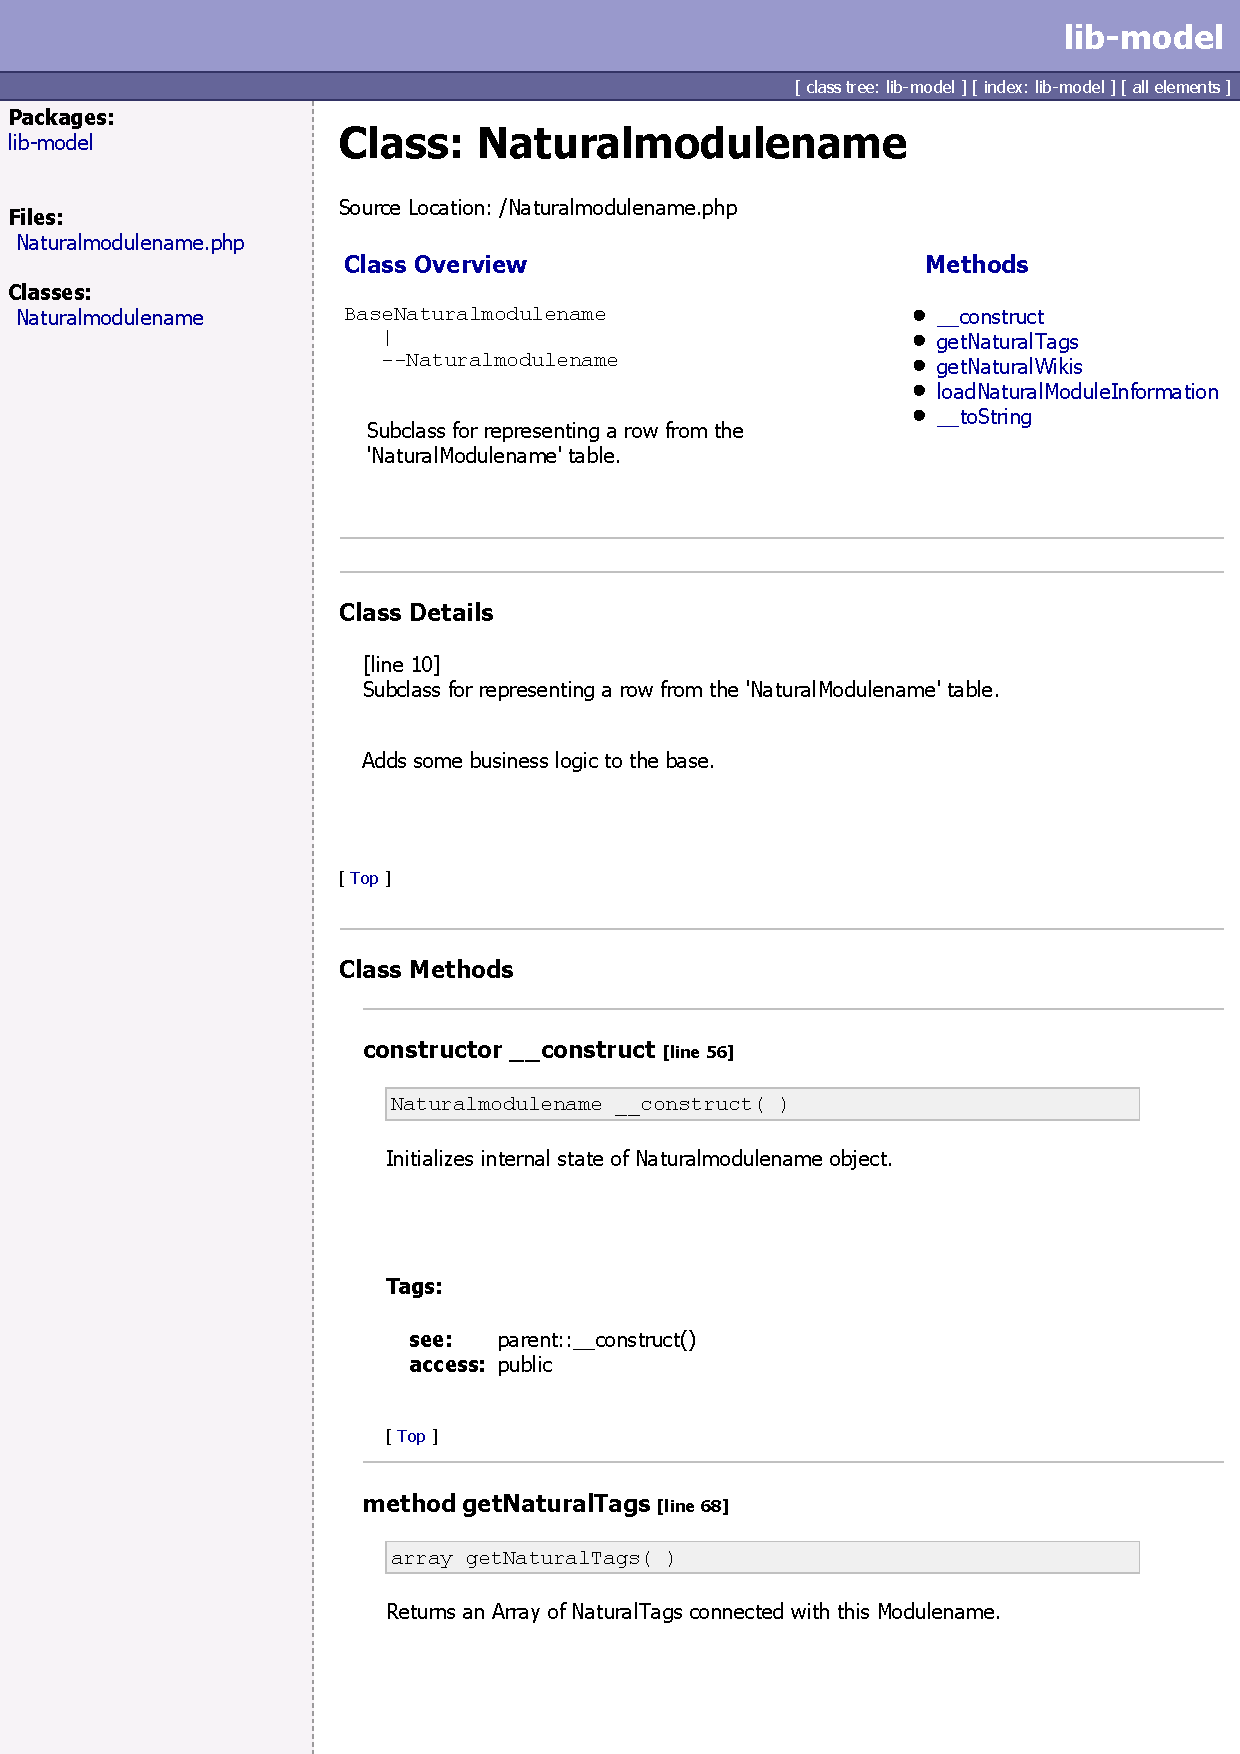
\includegraphics[page=1, width=0.9\textwidth]{doc.pdf}

\includegraphics[page=2, width=0.9\textwidth]{doc.pdf}
\end{center}

\clearpage
\subsection{Testfall und sein Aufruf auf der Konsole}
\label{app:Test}
\lstinputlisting[language=php, caption={Testfall in PHP}]{Listings/tests.php}
\clearpage
\begin{figure}[htb]
\centering
\includegraphicsKeepAspectRatio{testcase.jpg}{1}
\caption{Aufruf des Testfalls auf der Konsole}
\end{figure}


\subsection{Klasse: ComparedNaturalModuleInformation}
\label{app:CNMI}
Kommentare und simple Getter/Setter werden nicht angezeigt.
\lstinputlisting[language=php, caption={Klasse: ComparedNaturalModuleInformation}]{Listings/cnmi.php}
\clearpage

\subsection{Klassendiagramm}
\label{app:Klassendiagramm}
Klassendiagramme und weitere \acs{UML}-Diagramme kann man auch direkt mit \LaTeX{} zeichnen, siehe \zB \url{http://metauml.sourceforge.net/old/class-diagram.html}.
\begin{figure}[htb]
\centering
\includegraphicsKeepAspectRatio{Klassendiagramm.pdf}{1}
\caption{Klassendiagramm}
\end{figure}
\clearpage

\subsection{Benutzerdokumentation}
\label{app:BenutzerDoku}
Ausschnitt aus der Benutzerdokumentation:

\begin{table}[htb]
\begin{tabularx}{\textwidth}{cXX}
\rowcolor{heading}\textbf{Symbol} & \textbf{Bedeutung global} & \textbf{Bedeutung einzeln} \\
\includegraphicstotab[]{weather-clear.png} & Alle Module weisen den gleichen Stand auf. & Das Modul ist auf dem gleichen Stand wie das Modul auf der vorherigen Umgebung. \\
\rowcolor{odd}\includegraphicstotab[]{weather-clear-night.png} & Es existieren keine Module (fachlich nicht möglich). & Weder auf der aktuellen noch auf der vorherigen Umgebung sind Module angelegt. Es kann also auch nichts übertragen werden. \\
\includegraphicstotab[]{weather-few-clouds-night.png} & Ein Modul muss durch das Übertragen von der vorherigen Umgebung erstellt werden. & Das Modul der vorherigen Umgebung kann übertragen werden, auf dieser Umgebung ist noch kein Modul vorhanden. \\
\rowcolor{odd}\includegraphicstotab[]{weather-few-clouds.png} & Auf einer vorherigen Umgebung gibt es ein Modul, welches übertragen werden kann, um das nächste zu aktualisieren. & Das Modul der vorherigen Umgebung kann übertragen werden um dieses zu aktualisieren. \\
\includegraphicstotab[]{weather-storm.png} & Ein Modul auf einer Umgebung wurde entgegen des Entwicklungsprozesses gespeichert. & Das aktuelle Modul ist neuer als das Modul auf der vorherigen Umgebung oder die vorherige Umgebung wurde übersprungen. \\
\end{tabularx}
\end{table}




\end{document}
